\section{Experiments}
\label{sec:exp}

\subsection{Data Collection}
\label{sec:datacollection}

We are using ROpenDota by Rosdyana Kusuma to built our data set. ROpenDota is an API wrapper service for OpenDota in R. We labeling players from replay and the replay based on The International 2016 and Kiev Major, which contains 8419 labeled players. Using replay data from professional players will guarantee our data set from low-level data.

\subsection{Attribute Construction and Evaluation}
\label{sec:attconsandeval}

Attributes for evaluation is presented in table \ref{table:table1}. While some attributes correspond directly to summary data, attributes that capture positional information the fighting behavior require more complex processing of the replay data. Different attribute filters implemented in the Java library WEKA \cite{hall2009weka} to determine the best set of attributes. Our results with the \textit{WrapperSubsetEval} class with best-first search are presented in table 1. We have chosen this algorithm for our final attribute selection because it resulted in the highest accuracy with our labeled data set. For classification, we selected all attributes that were present in at least four folds, excluding assists, as this resulted in the overall highest accuracy. In the following sections, we describe the algorithms and heuristics we developed to calculate the attributes that cannot be directly obtained from replay files. They can be grouped into five rough categories: space and movement, early ganks, team fights, support items, and damage types. Not all of the attributes we describe in this section were finally chosen to be used for classification within this work but they might prove valuable for future works.

\begin{figure}
\centering
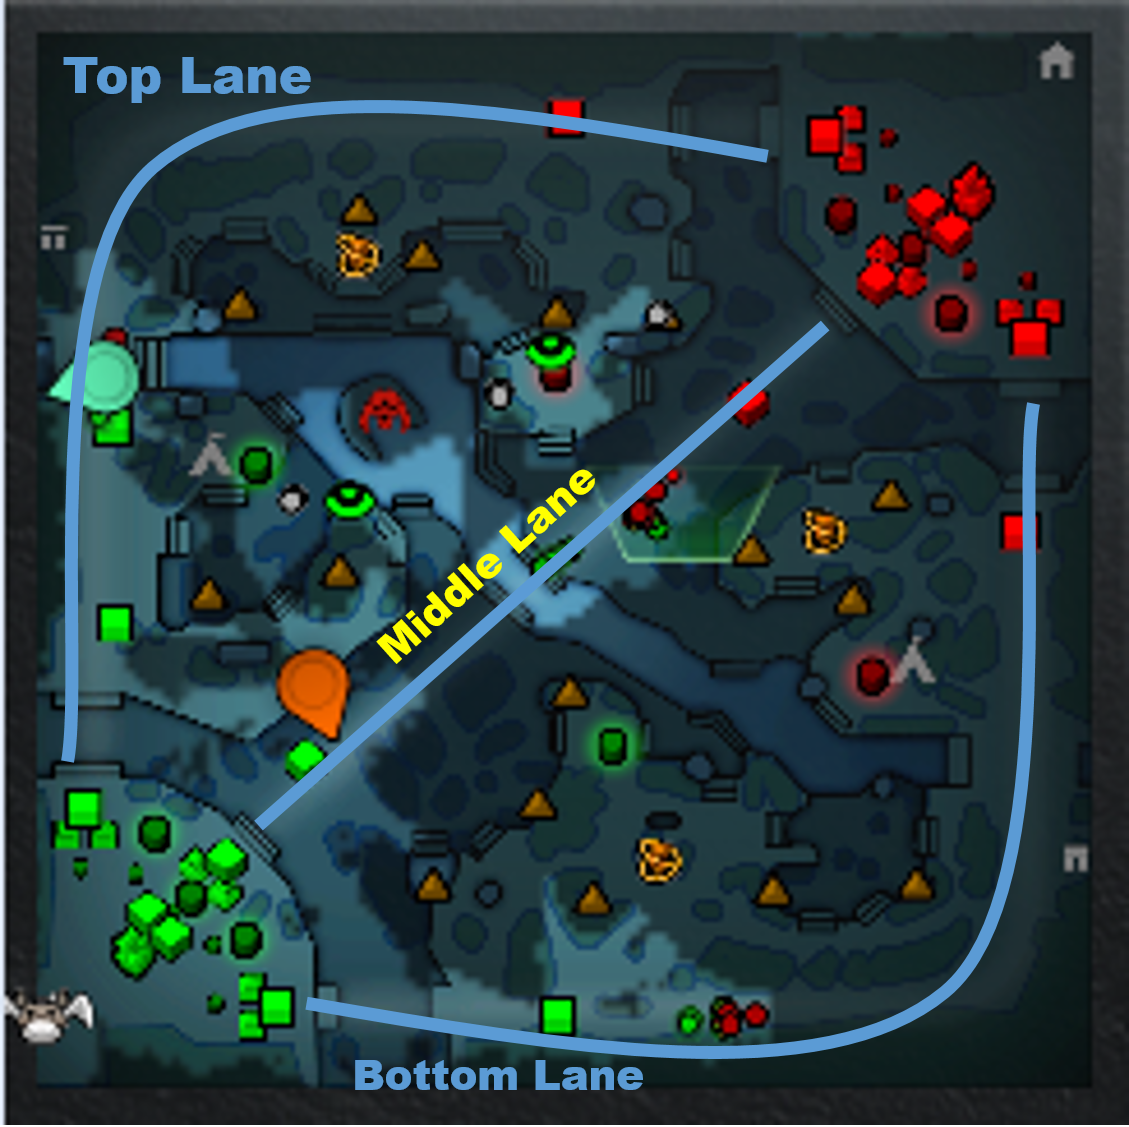
\includegraphics[width=1.5in]{./figures/lane_map.png}
\caption{\textit{Dota 2} map designed with three lane. Top lane, middle lane and also bottom lane.}
\label{fig:map_lane}
\end{figure}

\textbf{Player Lane} Most of the player roles depend on the lane (see figure \ref{fig:map_lane}) which is the most active in the early game. Player lane information also provides the constructor for the other attributes, e.g., the \textit{lane partners}. In the early game, players commonly have three main positions: \textit{top lane}, \textit{mid lane}, or \textit{bottom lane}. In additional, the \textit{jungle} areas also can be used ( see figure \ref{fig:map_jungle}). Or, players can have a \textit{roaming} position, it means that they will move around the map instead of focusing in a specific lane.

\begin{figure}
\centering
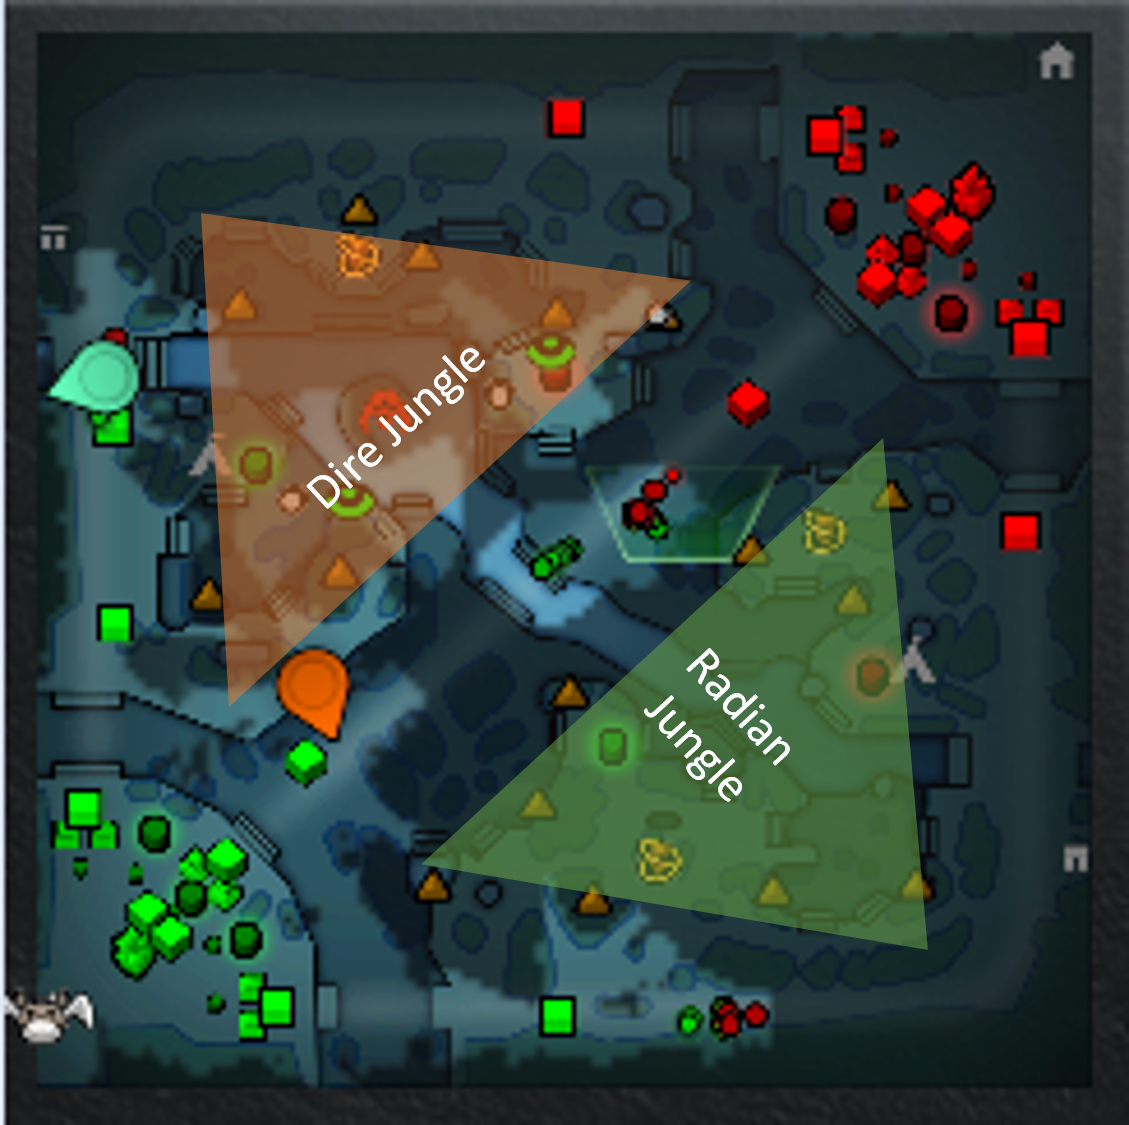
\includegraphics[width=1.5in]{./figures/map_jungle.png}
\caption{\textit{Dota 2} map jungle areas divided into two areas, \textit{Dire} and \textit{Radiant} jungle.}
\label{fig:map_jungle}
\end{figure}

\renewcommand{\arraystretch}{1.5}
\setlength{\tabcolsep}{12pt}
\begin{table}[]
\caption{Attributes evaluated for classification. Attributes marked with + are not directly available from replays. Attributes marked with {*} were finally selected for classification. Number of Folds shows in how many folds an attribute was selected by WEKA’s WrapperSubsetEval class using 10-fold cross-validation for each classification.}
\label{table:table1}
\centering
\begin{tabular}{|c|c|}
\hline
\textbf{Attribute}                            & \textbf{Number of Folds} \\ \hline
KDA Ratio* = (Kills + Assists) / (Deaths + 1) & 10                       \\ \hline
Last Hits*                                    & 10                       \\ \hline
Early Ganks*+                                 & 10                       \\ \hline
Number of Support Items*+                     & 10                       \\ \hline
Damage to Neutral Creeps*+                    & 10                       \\ \hline
Damage to Regular Creeps*+                    & 10                       \\ \hline
Lane Partners*+                               & 10                       \\ \hline
Kills*                                        & 9                        \\ \hline
Experience*                                   & 5                        \\ \hline
Deaths*                                       & 5                        \\ \hline
Assists                                       & 5                        \\ \hline
Team Fight Participation*+                    & 4                        \\ \hline
Early Movement (Visited Cells)*+              & 4                        \\ \hline
Damage to Heroes*+                            & 4                        \\ \hline
Solo Lane+                                    & 2                        \\ \hline
Damage to Towers+                             & 1                        \\ \hline
Chosen Hero                                   & 0                        \\ \hline
Gold                                          & 0                        \\ \hline
\end{tabular}
\end{table}

\textbf{Lane Partners and Solo Lane} To calculate the lane attribute from lane partners and solo lane can be determined by comparing the number of players. The player in \textit{jungle} position or \textit{roaming} are always assigned with zero lane partners, while players who are sharing the other lane, such as top, mid or bottom lane are corresponding with a number of their \textit{teammates} in the current lane. Solo lane attribute included in our attributes as an alternative to the lane partners. The value of this attribute will be true if a player is assigned to one of the tree main lanes without any teammate and otherwise false.

\textbf{Support Items} Player who considering playing as support mostly must buy support items. Many items in \textit{Dota 2} are useful for support player. List of common suppor items: \textit{Courier}, \textit{Flying Courier}, \textit{Observer Ward} and \textit{Sentry Ward}. 

\textbf{Damage Types} We categorized damage type based on player roles and requirement of other attributes: damage to the tower, damage to heroes, damage to regular creeps, damage to neutral creeps and damage to ancient creeps.

\subsection{Feature Normalization}
\label{sec:featurenorm}

An approach of \textit{Feature Normalization} to enhance the accuracy result proved by Singh \cite{singh2015investigations}. We applied feature normalization on this paper to cross check if this methodology can help to tweak accuracy of classification results. Various normalization techniques in this study are:

\textbf{Z-Score Normalization}, A very common techniques to normalize the feature to zero mean and unit variance is Z-score normalization \cite{jayalakshmi2011statistical}. It is a linear technique which initially mean ( \(\bar{x}\) ) and standard deviation ( \(\sigma\) ) of the specific feature values are computed using:

\begin{equation}
\bar{x}=\frac{1}{N}\sum_{i-1}^{N}x_{i}
\end{equation}

and,
\begin{equation}
\sigma^2=\frac{1}{N-1}\sum_{i-1}^{N}(x_{i}-\bar{x})^2
\end{equation}

the normalized feature is then given by:
\begin{equation}
\bar{x}_i=\frac{x_i-\bar{x}}{\sigma}
\end{equation}

\textbf{Min-Max Normalization}, This technique performs a linear transformation on the original data. For mapping a value, of an attribute \(x_i\) from range [min(\(x_i\)), max(\(x_i\))] to a new range [min \(x_new,\),max \(x_new\), the normalized feature is given by:

\begin{equation}
\hat{x}_i=\frac{X_i-min(x_i)}{max(x_i)-min(x_i)}
\end{equation}

The advantage of Min-Max normalization is that it preserves the relationship among the original data values \cite{manikandan2013achieving}. In this study \(max\,x_{new}=1\) and \(min\,x_{new}=-1\) is used.

\textbf{Linar Scaling to Unit Range}, This is also a linear transformation technique to normalize data in range[0,1]. Given a lower bound min(\(x_i\)) and upper bound max(\(x_i\)) of an attribute \(x_i\), the normalized value is given by:

\begin{equation}
\hat{x}_i=\frac{x_i-min(x_i)}{max(x_i)-min(x_i)}
\end{equation}

Linear scaling to unit range is special case of min-max normalization in which max\(\,x_{new}\)=1 and min\(\,x_{new}\)=0.

\textbf{Softmax Scaling}, In addition to linear scaling, nonlinear normalization techniques may be used in cases where data are not evenly distributed around the mean \cite{theodoridis2010introduction}. In such cases, the transformations based on nonlinear (i.e., exponential, logarithmic, sigmoid etc) functions can be used to map the data within specified intervals. One such popular technique is so called softmax scaling which squashes the data value non linearly in the interval [0,1]. the normalized feature is given by:

\begin{equation}
\hat{x}_i=\frac{1}{1+e^{-y}}
\end{equation}

where \(y=\frac{x_i-\bar{x}}{r\sigma}\) and \textit{r} is a user defined parameter. in the above equation that for small values of y i.e., for values of \(x_i\) closer to mean, y is an approximately linear function. Values away from mean are squashed exponentially.